% ============================================================
%  يُترجَم بـ XeLaTeX  (في Overleaf: Menu → Compiler → XeLaTeX)
%  الخط: Amiri (متوفر في Overleaf، أو حمّله من github.com/aliftype/amiri)
% ============================================================
\documentclass[12pt,a4paper]{article}
\usepackage[a4paper,margin=1.7cm,top=2.3cm,bottom=2.9cm,headheight=15pt,footskip=1.5cm]{geometry}
\usepackage{amsmath,amssymb}
\usepackage{icomma}
\usepackage[english,bidi=default,layout=lists]{babel}
\babelprovide[import,main]{arabic}
\babelfont{rm}[Scale=1.08]{Amiri}
\babelfont{sf}[Scale=1.08]{Amiri}
\usepackage[most]{tcolorbox}
\usepackage{tikz}
\usetikzlibrary{arrows.meta,calc,shadings}
\usepackage{array}
\usepackage{colortbl}
\usepackage{fancyhdr}
\usepackage{titlesec}
\usepackage{enumitem}
\usepackage{collcell}
\usepackage{needspace}
\usepackage{etoolbox}
% أعمدة جداول تُكتب خلاياها بالعربية في الاتجاه الصحيح
\newcolumntype{C}{>{\collectcell\ar}c<{\endcollectcell}}
% تجنب عنوان يتيم في أسفل الصفحة
\pretocmd{\section}{\Needspace{15\baselineskip}}{}{}
\pretocmd{\subsection}{\Needspace{11\baselineskip}}{}{}

% ---------- الألوان ----------
\definecolor{cDef}{HTML}{1F4E9C}
\definecolor{cThm}{HTML}{B3261E}
\definecolor{cRem}{HTML}{2E7D32}
\definecolor{cEx}{HTML}{C76B00}
\definecolor{cMeth}{HTML}{6A1B9A}
\definecolor{cSol}{HTML}{00695C}
\definecolor{cSec}{HTML}{1F3A68}

% ---------- العناوين ----------
\titleformat{\section}{\Large\bfseries\color{cSec}}{\thesection.}{0.6em}{}[{\color{cSec!60}\titlerule[1pt]}]
\titleformat{\subsection}{\large\bfseries\color{cThm!85!black}}{\thesubsection.}{0.5em}{}
\titlespacing*{\section}{0pt}{14pt}{8pt}
\titlespacing*{\subsection}{0pt}{10pt}{5pt}
\setlength{\parindent}{0pt}
\setlength{\parskip}{4pt}
\setlist{itemsep=2pt,topsep=3pt}

% ---------- الصناديق (تُرسم في سياق LTR ويُكتب محتواها بالعربية) ----------
\newtcolorbox{arbox}[3][]{enhanced,
  colback=#2!5,colframe=#2!80!black,arc=2mm,boxrule=0.8pt,
  left=6pt,right=6pt,top=8pt,bottom=5pt,
  fonttitle=\bfseries,coltitle=white,
  title={\foreignlanguage{arabic}{#3}},
  attach boxed title to top right={xshift=-5mm,yshift=-3mm},
  boxed title style={colback=#2!80!black,arc=1.5mm,boxrule=0pt},
  before upper={\selectlanguage{arabic}},
  before skip=8pt,after skip=8pt,breakable,#1}
\newenvironment{BOX}[2]{\begin{otherlanguage}{english}\begin{arbox}{#1}{#2}}{\end{arbox}\end{otherlanguage}}
\newenvironment{tarif}[1][تعريف]{\begin{BOX}{cDef}{#1}}{\end{BOX}}
\newenvironment{khassia}[1][خاصية]{\begin{BOX}{cThm}{#1}}{\end{BOX}}
\newenvironment{molahada}[1][ملاحظة]{\begin{BOX}{cRem}{#1}}{\end{BOX}}
\newenvironment{mithal}[1][مثال]{\begin{BOX}{cEx}{#1}}{\end{BOX}}
\newenvironment{tariqa}[1][طريقة]{\begin{BOX}{cMeth}{#1}}{\end{BOX}}

% ---------- التمارين والحلول ----------
\newcounter{exo}
\newenvironment{tamrin}[1]{\stepcounter{exo}\begin{BOX}{cSec}{التمرين \theexo: #1}}{\end{BOX}}
\newenvironment{hal}{\Needspace{12\baselineskip}\begin{otherlanguage}{english}\begin{arbox}[breakable]{cSol}{حل التمرين \theexo}}{\end{arbox}\end{otherlanguage}}

% رسومات TikZ تُوضع في سياق LTR
\newenvironment{LTR}{\begin{otherlanguage}{english}}{\end{otherlanguage}}
\newcommand{\ar}[1]{\foreignlanguage{arabic}{#1}}

% ---------- رموز ----------
% نقاط الحذف داخل الرياضيات (\dots يسبب خللاً في الاتجاه مع babel)
\renewcommand{\dots}{\mathinner{\ldotp\ldotp\ldotp}}
\renewcommand{\ldots}{\mathinner{\ldotp\ldotp\ldotp}}
\renewcommand{\cdots}{\mathinner{\cdotp\cdotp\cdotp}}
\newcommand{\N}{\mathbb{N}}
\newcommand{\Z}{\mathbb{Z}}
\newcommand{\D}{\mathbb{D}}
\newcommand{\Q}{\mathbb{Q}}
\newcommand{\R}{\mathbb{R}}
\newcommand{\pgcd}{\operatorname{PGCD}}
\newcommand{\ppcm}{\operatorname{PPCM}}

% ---------- تمثيل مجال على مستقيم عددي ----------
% \NLseg{a}{b}{[}{]}  مجال محدود
\newcommand{\NLseg}[4]{\begin{LTR}\begin{tikzpicture}[baseline=-0.6ex]
 \draw[-{Stealth[length=2mm]},gray!70](0,0)--(3.4,0);
 \draw[line width=2pt,cThm!80!black](0.7,0)--(2.7,0);
 \node[cThm!80!black,font=\LARGE] at (0.7,0){$#3$};
 \node[cThm!80!black,font=\LARGE] at (2.7,0){$#4$};
 \node[below=3pt,font=\footnotesize] at (0.7,0){$#1$};
 \node[below=3pt,font=\footnotesize] at (2.7,0){$#2$};
\end{tikzpicture}\end{LTR}}
% \NLright{a}{[}  مجال نحو +∞
\newcommand{\NLright}[2]{\begin{LTR}\begin{tikzpicture}[baseline=-0.6ex]
 \draw[-{Stealth[length=2mm]},gray!70](0,0)--(3.4,0);
 \draw[line width=2pt,cThm!80!black](1.3,0)--(3.3,0);
 \node[cThm!80!black,font=\LARGE] at (1.3,0){$#2$};
 \node[below=3pt,font=\footnotesize] at (1.3,0){$#1$};
\end{tikzpicture}\end{LTR}}
% \NLleft{b}{]}  مجال نحو −∞
\newcommand{\NLleft}[2]{\begin{LTR}\begin{tikzpicture}[baseline=-0.6ex]
 \draw[-{Stealth[length=2mm]},gray!70](0,0)--(3.4,0);
 \draw[line width=2pt,cThm!80!black](0.05,0)--(2.1,0);
 \node[cThm!80!black,font=\LARGE] at (2.1,0){$#2$};
 \node[below=3pt,font=\footnotesize] at (2.1,0){$#1$};
\end{tikzpicture}\end{LTR}}

% ---------- أيقونات مواقع التواصل (مرسومة بـ TikZ، لا تحتاج أي حزمة) ----------
\definecolor{cFB}{HTML}{1877F2}
\definecolor{cTG}{HTML}{229ED9}
\definecolor{cIG1}{HTML}{FEDA75}
\definecolor{cIG2}{HTML}{D62976}
\definecolor{cIG3}{HTML}{4F5BD5}
\newcommand{\fbicon}{\begin{LTR}\begin{tikzpicture}[baseline=-0.75ex,x=1em,y=1em]
 \fill[cFB] (0,0) circle (0.55);
 \node[white,inner sep=0,font=\usefont{TU}{lmss}{bx}{n}\small] at (0.04,-0.02) {f};
\end{tikzpicture}\end{LTR}}
\newcommand{\igicon}{\begin{LTR}
\begin{tikzpicture}[baseline=-0.75ex,x=1em,y=1em]
 \shade[lower left=cIG1,lower right=cIG2,upper left=cIG2,upper right=cIG3,rounded corners=0.28em] (-0.55,-0.55) rectangle (0.55,0.55);
 \draw[white,line width=0.09em,rounded corners=0.18em] (-0.36,-0.36) rectangle (0.36,0.36);
 \draw[white,line width=0.09em] (0,0) circle (0.17);
 \fill[white] (0.22,0.22) circle (0.05);
\end{tikzpicture}\end{LTR}}
\newcommand{\tgicon}{\begin{LTR}
\begin{tikzpicture}[baseline=-0.75ex,x=1em,y=1em]
 \fill[cTG] (0,0) circle (0.55);
 \fill[white] (-0.33,0.0) -- (0.32,0.27) -- (0.2,-0.3) -- (0.0,-0.15) -- (-0.08,-0.28) -- (-0.08,-0.08) -- cycle;
 \fill[cTG!70!black] (-0.08,-0.08) -- (0.25,0.2) -- (0.0,-0.15) -- (-0.08,-0.28) -- cycle;
\end{tikzpicture}\end{LTR}}
% سطر مواقع التواصل أسفل كل صفحة
% (يُكتب السطر بترتيب بصري من اليسار إلى اليمين: الأيقونة يمين كل اسم)
\newcommand{\PageBox}{\begin{LTR}\tikz[baseline=(p.base)]\node[fill=black,text=white,inner sep=2.5pt,minimum width=1.6em,minimum height=1.3em,font=\usefont{TU}{lmss}{bx}{n}\small](p){\ifnum\value{page}<10 0\fi\arabic{page}};\end{LTR}}
\newcommand{\SocialRow}{\begin{otherlanguage}{english}%
 \ar{\textbf{الأستاذ سوايسية هشام للرياضيات}}\ \tgicon\hfill
 \textbf{prof\_hicham\_math}\ \igicon\hfill
 \ar{\textbf{الأستاذ سوايسية هشام للرياضيات}}\ \fbicon\hspace{2.2em}\PageBox\end{otherlanguage}}
% ---------- رأس وتذييل الصفحة ----------
\pagestyle{fancy}
\fancyhf{}
\renewcommand{\headrulewidth}{0.6pt}
\renewcommand{\footrulewidth}{0.4pt}
% \SetHeader{يمين الرأس}{يسار الرأس}{يمين التذييل}{يسار التذييل}
\newcommand{\SetHeader}[2]{%
 \fancyhead[C]{\parbox{\textwidth}{\ar{#1\hfill #2}}}%
 \fancyfoot[C]{\parbox{\textwidth}{\small\SocialRow}}}

\usepackage{tkz-tab}
\usepackage{multicol}
% جدول تغيرات / إشارة (يُرسم في سياق LTR)
\newenvironment{TAB}{\par\begin{center}\begin{LTR}\begin{tikzpicture}[scale=0.95,every node/.style={font=\small}]}{\end{tikzpicture}\end{LTR}\end{center}}
% معلم بشبكة: \begin{GR}{xmin}{xmax}{ymin}{ymax}{unit cm}
\newenvironment{GR}[5]{\par\begin{center}\begin{LTR}\begin{tikzpicture}[x=#5cm,y=#5cm,font=\footnotesize]
 \def\xmn{#1}\def\xmx{#2}\def\ymn{#3}\def\ymx{#4}
 \draw[gray!25,very thin] (#1,#3) grid (#2,#4);
 \draw[-{Stealth[length=2mm]}] (#1,0)--(#2+0.3,0) node[below left]{$x$};
 \draw[-{Stealth[length=2mm]}] (0,#3)--(0,#4+0.3) node[below left]{$y$};
 \node[below left] at (0,0){$O$};
 \draw[very thick,-{Stealth[length=1.6mm]}] (0,0)--(1,0) node[below,pos=.55]{$\vec i$};
 \draw[very thick,-{Stealth[length=1.6mm]}] (0,0)--(0,1) node[left,pos=.55]{$\vec j$};
 \begin{scope}\clip (#1,#3) rectangle (#2,#4);}
{\end{scope}\end{tikzpicture}\end{LTR}\end{center}}
\newcommand{\Ticks}[2]{\foreach \t in {#1} \node[below,font=\scriptsize] at (\t,0){$\t$}; \foreach \t in {#2} \node[left,font=\scriptsize] at (0,\t){$\t$};}
\newcommand{\bx}[1]{\ensuremath{\colorbox{cDef!12}{$\displaystyle #1$}}}
\newtcbox{\bxtbox}{on line,colback=cDef!12,colframe=cDef!12,boxrule=0pt,arc=1pt,boxsep=0pt,left=2pt,right=2pt,top=1pt,bottom=1pt}
\newcommand{\bxt}[1]{\foreignlanguage{english}{\bxtbox{\ar{#1}}}}
\newcommand{\hl}[1]{\ensuremath{\colorbox{cEx!20}{$\displaystyle #1$}}}
\newcommand{\Lim}[1]{\displaystyle\lim_{x\to #1}}
\newcommand{\Cf}{(C_f)}
\newenvironment{qst}{\begin{enumerate}[label=\protect\circled{\arabic*},leftmargin=*]}{\end{enumerate}}
\newcommand{\circled}[1]{\foreignlanguage{english}{\tikz[baseline=(c.base)]\node[circle,fill=cDef,text=white,inner sep=1.2pt,font=\scriptsize\bfseries](c){#1};}}
% عمودان: \TwoCol{عرض اليسار}{محتوى اليسار}{عرض اليمين}{محتوى اليمين}  (آمن مع TikZ)
\newcommand{\TwoCol}[4]{\par\begin{LTR}\noindent\begin{minipage}[t]{#1\textwidth}\selectlanguage{arabic}#2\end{minipage}\hfill\begin{minipage}[t]{#3\textwidth}\selectlanguage{arabic}#4\end{minipage}\end{LTR}\par}
\newcommand{\un}{(u_n)}\newcommand{\vn}{(v_n)}
\newcommand{\src}[1]{{\footnotesize\textbf{#1}}\par}
\newcommand{\ok}{$\textcolor{cRem}{\checkmark}$}
\newcommand{\limn}{\displaystyle\lim_{n\to+\infty}}
% أسئلة فرعية (أ) (ب) (جـ) كل سؤال في سطر
\newenvironment{sq}{\begin{itemize}[leftmargin=2.4em,itemsep=3pt]}{\end{itemize}}
\newcommand{\qa}{\item[(أ)]}\newcommand{\qb}{\item[(ب)]}\newcommand{\qc}{\item[(جـ)]}\newcommand{\qd}{\item[(د)]}\newcommand{\qe}{\item[(هـ)]}
\newcommand{\pa}{\par\smallskip\textbf{(أ)} }\newcommand{\pb}{\par\smallskip\textbf{(ب)} }\newcommand{\pc}{\par\smallskip\textbf{(جـ)} }\newcommand{\pd}{\par\smallskip\textbf{(د)} }\newcommand{\pe}{\par\smallskip\textbf{(هـ)} }
\newcommand{\ccl}[1]{\par\textbf{الخلاصة:} #1}

\pretocmd{\section}{\Needspace{24\baselineskip}}{}{}
\SetHeader{\small\bfseries\color{cSec}تمارين: المتتاليات العددية}{\small\color{cSec}السنة الثانية ثانوي -- الشعب العلمية}
\begin{document}
\newcolumntype{M}[1]{>{\centering\arraybackslash}p{#1}}
\newcommand{\RL}[4]{\TwoCol{#3}{#4}{#1}{#2}}
\newcommand{\QQ}[1]{\par\smallskip\textbf{#1.} }
\newcommand{\Un}{(u_n)}
\newcommand{\ABC}[3]{\\[2pt]\begin{tabular}{p{0.28\textwidth}p{0.28\textwidth}p{0.28\textwidth}}(جـ) \ #3 & (ب) \ #2 & (أ) \ #1\end{tabular}}
\begin{LTR}
\begin{tcolorbox}[enhanced,colback=cSec,colframe=cSec,arc=3mm,halign=center,boxrule=0pt,top=12pt,bottom=12pt,before upper={\selectlanguage{arabic}}]
{\color{white}\fontsize{26}{32}\selectfont\bfseries سلسلة تمارين: المتتاليات العددية}\\[8pt]
{\color{white}\large تمارين متنوعة ومسائل شاملة -- بدون حلول (للتدرّب)}\\[5pt]
{\color{white}\large السنة الثانية ثانوي -- الشعب العلمية}
\end{tcolorbox}
\end{LTR}

% =====================================================================
\section{عموميات: التوليد ، اتجاه التغير والتمثيل البياني}
% ------------------------------------------------- 1
\begin{tamrin}{حساب حدود وطرق التوليد}
\begin{enumerate}
\item احسب الحدود الثلاثة الأولى لكل متتالية مما يلي (عيّن أولاً مجموعة تعريفها):
\begin{sq}
\qa $u_n=n^3-3$
\qb $v_n=\dfrac{-1}{n}$
\qc $w_n=\dfrac{n+3}{n-2}$
\qd $c_n=\sqrt{n-4}$
\end{sq}
\item $\Un$ متتالية معرّفة بـ $u_n=3n+5$. \ عيّن الدالة المرفقة بها ، ثم احسب $u_{20}$ ورتبته.
\item $(t_n)$ متتالية معرّفة على $\N$ بـ: $t_0=1$ و $t_{n+1}=2t_n+1$. \ احسب $t_1$ ، $t_2$ و $t_3$ ، ثم عيّن الدالة المرفقة.
\end{enumerate}
\end{tamrin}

% ------------------------------------------------- 2
\begin{tamrin}{دراسة اتجاه التغير بثلاث طرق وابتداءً من رتبة معيّنة}
ادرس اتجاه تغير كل متتالية مما يلي:
\begin{sq}
\qa $u_n=n^2+n$ \ ($n\in\N$) \ (بإشارة الفرق).
\qb $v_n=\dfrac{3^n}{n+4}$ \ ($n\in\N$) \ (بالنسبة $\dfrac{v_{n+1}}{v_n}$).
\qc $w_n=-2n+3$ \ ($n\in\N$) \ (بالدالة المرفقة ، ثم بإشارة الفرق).
\qd $t_n=\dfrac{2n+1}{n+3}$ \ ($n\in\N$) \ (بالدالة المرفقة).
\qe $s_n=n^2-8n+3$ \ ($n\in\N$): \ احسب $s_{n+1}-s_n$ ، ثم بيّن أن $(s_n)$ متزايدة تماماً ابتداءً من رتبة $n_0$ يطلب تعيينها. \ هل $(s_n)$ متزايدة على $\N$؟
\end{sq}
\end{tamrin}

% ------------------------------------------------- 3
\begin{tamrin}{تمثيل بياني ، متتالية هندسية مساعدة واتجاه التغير}
\RL{0.6}{%
في المستوي المنسوب إلى معلم متعامد ومتجانس ، $(\Delta)$ و $(D)$ مستقيمان معادلتاهما على الترتيب: $y=\dfrac12x+\dfrac13$ و $y=x$.\par
$\Un$ المتتالية المعرّفة على $\N$ بـ: $u_0=6$ ، ومن أجل كل $n$: $u_{n+1}=\dfrac12u_n+\dfrac13$.}{0.37}{%
\begin{LTR}\centering
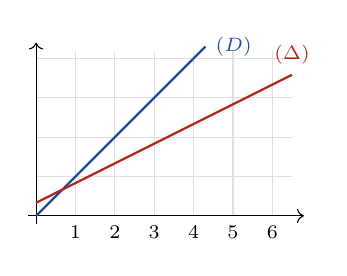
\begin{tikzpicture}[scale=0.5,font=\scriptsize]
\draw[gray!25] (0,0) grid (6.5,4.2);
\draw[->] (-0.2,0)--(6.8,0); \draw[->] (0,-0.2)--(0,4.4);
\draw[cDef,thick] (0,0)--(4.3,4.3) node[right]{$(D)$};
\draw[cThm,thick] (0,0.333)--(6.5,3.583) node[above]{$(\Delta)$};
\foreach \x in {1,...,6} \node[below] at (\x,0){$\x$};
\end{tikzpicture}
\end{LTR}}
\begin{enumerate}
\item
\begin{sq}
\qa مثّل على محور الفواصل الحدود $u_0$ ، $u_1$ ، $u_2$ ، $u_3$ و $u_4$ دون حسابها ، مبرزاً خطوط الإنشاء.
\qb عيّن إحداثيي نقطة تقاطع $(\Delta)$ و $(D)$.
\qc أعط تخميناً حول اتجاه تغير $\Un$.
\end{sq}
\item نعتبر المتتالية $(v_n)$ المعرّفة من أجل كل $n$ بـ: $v_n=u_n-\dfrac23$.
\begin{sq}
\qa بيّن أن $(v_n)$ هندسية يطلب تحديد أساسها وحدها الأول.
\qb اكتب $v_n$ ثم $u_n$ بدلالة $n$ ، واستنتج $\limn u_n$.
\qc احسب بدلالة $n$ المجموع $S_n=v_0+v_1+\cdots+v_n$ ، واستنتج $S'_n=u_0+u_1+\cdots+u_n$.
\end{sq}
\item
\begin{sq}
\qa احسب $u_{n+1}-u_n$ بدلالة $n$ ، ثم ادرس اتجاه تغير المتتالية $\Un$ (قارن مع التخمين).
\qb عيّن أصغر عدد طبيعي $n_0$ بحيث ابتداءً من الرتبة $n_0$ يكون: \ $u_n-\dfrac23<0{,}01$.
\end{sq}
\end{enumerate}
\end{tamrin}

% =====================================================================
\section{المتتاليات الحسابية}
% ------------------------------------------------- 4
\begin{tamrin}{متتالية حسابية ومجموع حدودها}
\begin{enumerate}
\item $\Un$ المتتالية المعرّفة على $\N$ بـ: $u_n=2n+5$.
\begin{sq}
\qa احسب $u_0$ ، $u_1$ و $u_2$.
\qb بيّن أن $\Un$ حسابية يطلب تعيين أساسها ، ثم استنتج اتجاه تغيرها.
\qc بيّن أن العدد $2025$ حد من حدود $\Un$ ، ثم استنتج رتبته.
\qd تحقق أن $u_0+u_1+\cdots+u_{1010}=1026165$ ، ثم احسب بدلالة $n$ المجموع $S_n=u_0+u_1+\cdots+u_n$.
\end{sq}
\item $(v_n)$ متتالية حسابية معرّفة على $\N$ بحدها الأول $v_0$ وأساسها $r$ ، حيث $v_3=13$ و $v_{10}=48$.
\begin{sq}
\qa عيّن $r$ و $v_0$.
\qb اكتب $v_n$ بدلالة $n$.
\end{sq}
\end{enumerate}
\end{tamrin}

% ------------------------------------------------- 5
\begin{tamrin}{الوسط الحسابي والمجاميع}
\begin{enumerate}
\item عيّن ثلاثة أعداد هي حدود متتابعة من متتالية حسابية ، مجموعها $15$ وجداؤها $80$.
\item عيّن العدد الحقيقي $x$ حتى تكون الأعداد $x-1$ ، $2x+1$ و $4x-1$ بهذا الترتيب حدوداً متتابعة من متتالية حسابية.
\item احسب المجاميع:
\begin{sq}
\qa $A=1+2+3+\cdots+1000$
\qb $B=1+\dfrac43+\dfrac53+2+\dfrac73+\cdots+11$
\qc $C=1+3+5+\cdots+99$
\end{sq}
\end{enumerate}
\end{tamrin}

% ------------------------------------------------- 6
\begin{tamrin}{متتالية تراجعية ومتتالية حسابية مساعدة}
$\Un$ متتالية عددية معرّفة على $\N$ بـ: $u_0=0$ و $u_{n+1}=\dfrac{u_n-1}{u_n+3}$.
\begin{enumerate}
\item بيّن أنه من أجل كل عدد طبيعي $n$: \ $u_{n+1}=1-\dfrac{4}{u_n+3}$.
\item احسب الحدود الخمسة الأولى للمتتالية $\Un$.
\item ادرس اتجاه تغير المتتالية $\Un$ علماً أنه من أجل كل $n$: $u_n\ge-1$.
\item نعتبر المتتالية $(v_n)$ المعرّفة على $\N$ بـ: $v_n=\dfrac{1}{u_n+1}$.
\begin{sq}
\qa بيّن أن $(v_n)$ متتالية حسابية يطلب تعيين أساسها وحدها الأول.
\qb اكتب عبارة $v_n$ بدلالة $n$ ، ثم استنتج عبارة $u_n$ بدلالة $n$.
\end{sq}
\end{enumerate}
\end{tamrin}

% =====================================================================
\section{المتتاليات الهندسية}
% ------------------------------------------------- 7
\begin{tamrin}{متتالية هندسية ومجموع حدودها}
\begin{enumerate}
\item $(V_n)$ متتالية هندسية معرّفة على $\N$ بـ: $V_n=5\times3^n$.
\begin{sq}
\qa احسب الحدود $V_0$ ، $V_1$ ، $V_2$ و $V_3$.
\qb تحقق أن $(V_n)$ هندسية أساسها $q=3$ وحدها الأول $V_0=5$.
\qc احسب المجموع $S_n=V_0+V_1+\cdots+V_n$.
\end{sq}
\item $(w_n)$ معرّفة على $\N$ بـ: $w_n=\dfrac{3}{2^n}$. \ بيّن أن $(w_n)$ هندسية يطلب تعيين أساسها وحدها الأول ، ثم ادرس اتجاه تغيرها.
\item $(t_n)$ هندسية حدها الأول $t_0=2$ وأساسها $q=3$. \ احسب بدلالة $n$ المجموع $t_0+t_1+\cdots+t_n$.
\end{enumerate}
\end{tamrin}

% ------------------------------------------------- 8
\begin{tamrin}{متتالية تراجعية من الشكل $u_{n+1}=au_n+b$}
نعتبر المتتالية $\Un$ المعرّفة على $\N$ بـ: $u_0=\alpha$ و $u_{n+1}=\dfrac23u_n+1$.
\begin{enumerate}
\item عيّن قيمة $\alpha$ حتى تكون المتتالية $\Un$ ثابتة.
\item نضع $u_0=6$.
\begin{sq}
\qa احسب الحدود $u_1$ ، $u_2$ و $u_3$ ، ثم ضع تخميناً حول اتجاه تغير $\Un$.
\qb بفرض أنه من أجل كل عدد طبيعي $n$: $u_n>3$ ، ادرس اتجاه تغير $\Un$.
\end{sq}
\item نعتبر المتتالية $(v_n)$ حيث: $v_n=u_n-3$.
\begin{sq}
\qa بيّن أن $(v_n)$ هندسية أساسها $q=\dfrac23$ يطلب تعيين حدها الأول $v_0$.
\qb اكتب $v_n$ بدلالة $n$ ، ثم استنتج $u_n$ بدلالة $n$.
\qc احسب المجموعين $S_n=v_0+v_1+\cdots+v_n$ و $S'_n=u_0+u_1+\cdots+u_n$.
\end{sq}
\end{enumerate}
\end{tamrin}

% ------------------------------------------------- 9
\begin{tamrin}{متتالية هندسية مساعدة ونهاية}
لتكن $\Un$ متتالية عددية معرّفة على $\N$ بحدها الأول $u_0=1$ ، ومن أجل كل $n$: $u_{n+1}=\dfrac13u_n+\dfrac13$. \ ولتكن $(v_n)$ المعرّفة بـ: $v_n=u_n-\dfrac12$.
\begin{enumerate}
\item احسب الحدود $u_1$ ، $u_2$ ، $u_3$ ، ثم ضع تخميناً حول اتجاه تغير $\Un$.
\item بيّن أن $(v_n)$ هندسية يطلب تعيين أساسها وحدها الأول $v_0$.
\item اكتب عبارة $v_n$ بدلالة $n$ ، ثم استنتج $u_n$ بدلالة $n$.
\item ادرس اتجاه تغير $(v_n)$ ، ثم استنتج اتجاه تغير $\Un$ ، واحسب $\limn u_n$.
\item احسب بدلالة $n$ المجموع $S_n=v_0+v_1+\cdots+v_n$ ، ثم استنتج $S'_n=u_0+u_1+\cdots+u_n$.
\end{enumerate}
\end{tamrin}

% ------------------------------------------------- 10
\begin{tamrin}{الوسط الهندسي}
\begin{enumerate}
\item عيّن ثلاثة أعداد هي حدود متتابعة من متتالية هندسية ، جداؤها $64$ ومجموعها $21$.
\item عيّن العدد الحقيقي الموجب $x$ حتى تكون الأعداد $x$ ، $x+2$ و $4x-1$ بهذا الترتيب حدوداً متتابعة من متتالية هندسية.
\end{enumerate}
\end{tamrin}

% =====================================================================
\section{وصف ظاهرة بواسطة متتالية}
% ------------------------------------------------- 11
\begin{tamrin}{إنتاج مصنع ونمو السكان}
\textbf{الجزء الأول:} أنتج مصنع في الشهر الأول $2000$ قارورة ، ويزيد إنتاجه كل شهر بـ $150$ قارورة عن الشهر الذي قبله. \ نسمي $u_n$ عدد القارورات المنتجة في الشهر رقم $n$ ($n\ge1$) ، أي $u_1=2000$.
\begin{sq}
\qa احسب $u_2$ و $u_3$.
\qb عبّر عن $u_{n+1}$ بدلالة $u_n$ ، واستنتج أن $\Un$ حسابية يطلب تعيين أساسها ، ثم اكتب $u_n$ بدلالة $n$.
\qc احسب إنتاج الشهر الثاني عشر ، ثم الإنتاج الإجمالي خلال السنة الأولى (الأشهر الـ $12$ الأولى).
\end{sq}
\textbf{الجزء الثاني:} عدد سكان مدينة $20000$ نسمة سنة $2025$ ، ويزداد كل سنة بنسبة $3\,\%$. \ نسمي $p_n$ عدد السكان سنة $2025+n$ ، أي $p_0=20000$.
\begin{sq}
\qa احسب $p_1$ و $p_2$.
\qb بيّن أن $(p_n)$ هندسية يطلب تعيين أساسها ، ثم اكتب $p_n$ بدلالة $n$.
\qc قدّر عدد السكان سنة $2035$.
\qd ادرس اتجاه تغير $(p_n)$ ، ثم عيّن باستعمال الآلة الحاسبة السنة التي يتجاوز فيها عدد السكان لأول مرة $30000$ نسمة.
\qe احسب $\limn p_n$. \ هل هذا النموذج صالح على المدى البعيد جداً؟
\end{sq}
\end{tamrin}

% =====================================================================
\section{نهاية متتالية}
% ------------------------------------------------- 12
\begin{tamrin}{حساب نهايات}
\begin{enumerate}
\item احسب نهاية كل متتالية مما يلي (عند $+\infty$):
\begin{sq}
\qa $a_n=\dfrac{2n+1}{n+3}$
\qb $b_n=\dfrac{n^2+1}{2n^2-n}$ \ ($n\ge1$)
\qc $c_n=-n^2+3n$
\qd $d_n=\Big(\dfrac{-3}{4}\Big)^n$
\qe $e_n=-2\times6^n$
\end{sq}
\item هل المتتالية $u_n=2+(-1)^n$ متقاربة؟ \ وهل $f_n=5\Big(\dfrac13\Big)^n+2$ متقاربة؟
\item $\Un$ متتالية حسابية حدها الأول $u_0=7$ وأساسها $3$. \ أوجد $u_n$ ، ثم احسب $S=u_0+u_1+\cdots+u_{200}$ ، وعيّن $\limn u_n$.
\end{enumerate}
\end{tamrin}

% =====================================================================
\section{مسائل شاملة}
% ------------------------------------------------- 13
\begin{tamrin}{متتالية هوموغرافية}
في الشكل ، $(C_f)$ هو تمثيل الدالة $f$ المعرّفة على $[0;5]$ بـ: $f(x)=\dfrac{4x-1}{x+2}$ ، و $(d)$ المستقيم ذو المعادلة $y=x$.\par
$\Un$ المتتالية المعرّفة بـ: $u_0=3$ ، ومن أجل كل $n$: $u_{n+1}=f(u_n)$.
\begin{enumerate}
\item مثّل على محور الفواصل الحدود $u_0$ ، $u_1$ ، $u_2$ و $u_3$ دون حسابها ، ثم أعط تخميناً حول اتجاه تغير $\Un$.
\item ادرس اتجاه تغير $\Un$ علماً أن $u_n>1$ من أجل كل $n$.
\item من أجل كل $n$ نضع: $v_n=\dfrac{1}{u_n-1}$.
\begin{sq}
\qa احسب $v_0$ ، ثم برهن أن $(v_n)$ حسابية أساسها $\dfrac13$.
\qb اكتب $v_n$ بدلالة $n$ ، ثم استنتج $u_n$ بدلالة $n$.
\qc احسب المجموع $S_n=v_0+v_1+\cdots+v_n$.
\end{sq}
\end{enumerate}
\end{tamrin}

% ------------------------------------------------- 14
\begin{tamrin}{متتالية تراجعية ومتتالية حسابية: مجموع معطى}
$\Un$ متتالية معرّفة بحدها الأول $u_0=2$ وبالعلاقة: $u_{n+1}=\dfrac{u_n}{2u_n+1}$. \ $(C_f)$ هو تمثيل الدالة $f(x)=\dfrac{x}{2x+1}$ على $\Big]-\dfrac12;+\infty\Big[$ ، و $(\Delta):y=x$.
\begin{enumerate}
\item
\begin{sq}
\qa مثّل على محور الفواصل الحدود $u_0$ ، $u_1$ و $u_2$ دون حسابها مبرزاً خطوط الرسم.
\qb ضع تخميناً حول اتجاه تغير $\Un$.
\qc إذا علمت أنه من أجل كل $n$: $u_n>0$ ، بيّن أن $\Un$ متناقصة تماماً.
\end{sq}
\item نعتبر المتتالية $(v_n)$ المعرّفة على $\N$ بـ: $v_n=\dfrac{1-u_n}{u_n}$ \ (حيث $u_n\ne0$).
\begin{sq}
\qa أثبت أن $(v_n)$ حسابية أساسها $2$ يطلب تعيين حدها الأول.
\qb اكتب $v_n$ بدلالة $n$ ، ثم استنتج أن $u_n=\dfrac{2}{4n+1}$.
\qc احسب بدلالة $n$ المجموع $S_n=\dfrac12v_0+\dfrac12v_1+\cdots+\dfrac12v_n$ ، ثم عيّن قيمة $n$ حتى يكون $S_n=2000$.
\end{sq}
\end{enumerate}
\end{tamrin}

% ------------------------------------------------- 15
\begin{tamrin}{متتاليتان متشابكتان}
نعتبر المتتاليتين $\Un$ و $(V_n)$ المعرّفتين بحديهما الأولين $U_0=2$ و $V_0=-1$ ، ومن أجل كل عدد طبيعي $n$ بالعلاقتين:
\[\begin{cases}U_{n+1}=(1+\alpha)U_n-\alpha V_n\\[2pt] V_{n+1}=(1-\alpha)U_n+\alpha V_n\end{cases}\qquad\text{\ar{حيث $\alpha$ وسيط حقيقي غير معدوم.}}\]
\begin{enumerate}
\item برهن باستعمال العلاقتين أنه إذا كانت $(U_n)$ متقاربة نحو $\ell$ فإن $(V_n)$ متقاربة كذلك نحو $\ell$.
\item نفرض أن $\alpha=\dfrac12$.
\begin{sq}
\qa بيّن أنه من أجل كل $n$: $U_n-V_n=3$ ، ثم استنتج أن $(U_n)$ حسابية يطلب تعيين أساسها.
\qb احسب بدلالة $n$ المجموع $S_n=U_0+U_1+\cdots+U_n$.
\end{sq}
\item نفرض أن $\alpha\ne\dfrac12$ ، ونعرّف المتتالية $(W_n)$ بـ: $W_n=U_n-V_n$.
\begin{sq}
\qa بيّن أن $(W_n)$ هندسية أساسها $q=2\alpha$.
\qb اكتب $W_n$ بدلالة $n$ و $\alpha$ ، ثم احسب المجموع $T_n=W_0+W_1+\cdots+W_n$.
\qc بيّن أنه من أجل كل $n\in\N$: \ $U_{n+1}-U_n=\alpha W_n$.
\qd استنتج أن: $U_n=\dfrac{3\times2^n\times\alpha^{n+1}+\alpha-2}{2\alpha-1}$.
\qe عيّن قيم $\alpha$ التي من أجلها تكون $(U_n)$ متقاربة ، ثم احسب نهايتها.
\end{sq}
\end{enumerate}
\end{tamrin}

% =====================================================================
\section{اختيار من متعدد ، صحيح أم خطأ}
% ------------------------------------------------- 16
\begin{tamrin}{اختيار من متعدد}
لكل سؤال جواب واحد صحيح من بين الأجوبة الثلاثة ، عيّنه مع التعليل:
\begin{enumerate}
\item $\Un$ حسابية حدها الأول $u_0=2$ وأساسها $r$ ، وتحقق: $u_0+\dfrac12u_4=u_3-1$. \ قيمة $r$ هي:
\ABC{$r=-2$}{$r=\dfrac12$}{$r=2$}
\item $(v_n)$ غير ثابتة معرّفة بـ: $v_{n+1}=(\alpha+1)v_n+1$. \ تكون $(v_n)$ حسابية من أجل:
\ABC{$\alpha=0$}{$\alpha=-1$}{$\alpha=1$}
\item $\Un$ هندسية ، $u_0=3$ و $q=2$. \ الحد $u_5$ يساوي:
\ABC{$30$}{$96$}{$192$}
\item المجموع $1+2+2^2+\cdots+2^{10}$ يساوي:
\ABC{$2047$}{$2048$}{$1023$}
\item $\Un$ حسابية حيث $u_5=17$ و $u_{12}=38$. \ أساسها هو:
\ABC{$3$}{$7$}{$-3$}
\item $\limn\Big(5\Big(\dfrac23\Big)^n+1\Big)$ تساوي:
\ABC{$+\infty$}{$1$}{$6$}
\item المتتالية $u_n=(-2)^n$:
\ABC{متزايدة}{متناقصة}{ليست رتيبة}
\item عدد الحدود من $u_7$ إلى $u_{40}$ هو:
\ABC{$33$}{$34$}{$40$}
\end{enumerate}
\end{tamrin}

% ------------------------------------------------- 17
\begin{tamrin}{صحيح أم خطأ}
أجب بصحيح أو خطأ مع التبرير:
\begin{enumerate}
\item إذا كانت المتتالية الحسابية $\Un$ متزايدة تماماً فإن أساسها أكبر تماماً من $0$.
\item $\Un$ متتالية حسابية أساسها $r=2$ ، لدينا $u_{n+1}=u_n-2$.
\item $\Un$ حسابية أساسها $r=2$ وحدها الأول $u_1=5$ ، عبارة حدها العام هي: $u_n=3+2n$.
\item $1+2+3+\cdots+999+1000=1001000$.
\item $\alpha$ عدد حقيقي غير معدوم ، و $(v_n)$ معرّفة بـ $v_0=1$ و $v_{n+1}=\dfrac1\alpha v_n$. \ قيمة $\alpha$ حتى تكون $(v_n)$ ثابتة هي $\alpha=2$.
\item $(w_n)$ حسابية أساسها $r=1$ وحدها الأول $w_1=2$. \ مجموع حدودها الـ $n$ الأولى هو $\dfrac{n(n+3)}{2}$.
\item كل متتالية هندسية أساسها $q=-2$ هي متتالية رتيبة.
\item إذا كان $u_n=f(n)$ و $f$ متزايدة على $[0;+\infty[$ فإن $\Un$ متزايدة.
\end{enumerate}
\end{tamrin}

% =====================================================================
\section{تمرين نموذجي}
% ------------------------------------------------- 18
\begin{tamrin}{تمرين نموذجي: متتالية متباعدة}
$\Un$ المتتالية المعرّفة على $\N$ بـ: $u_0=3$ و $u_{n+1}=3u_n-4$.
\begin{enumerate}
\item احسب $u_1$ ، $u_2$ و $u_3$. \ هل $\Un$ حسابية؟ هل هي هندسية؟
\item نضع $v_n=u_n-2$.
\begin{sq}
\qa بيّن أن $(v_n)$ هندسية يطلب تعيين أساسها وحدها الأول.
\qb اكتب $u_n$ بدلالة $n$ ، ثم احسب $\limn u_n$.
\qc عيّن أصغر عدد طبيعي $n$ حيث $u_n>1000$.
\qd احسب بدلالة $n$ المجموع $S'_n=u_0+u_1+\cdots+u_n$.
\end{sq}
\item ادرس اتجاه تغير $\Un$ بإشارة $u_{n+1}-u_n$.
\end{enumerate}
\end{tamrin}

\end{document}
